\documentclass[12pt,preprint]{article}
\usepackage[utf8]{inputenc}
\usepackage[T1]{fontenc}
\usepackage{amsmath,amssymb}
\usepackage{graphicx}
\usepackage{hyperref}
\usepackage{booktabs}
\usepackage{float}
\usepackage{placeins}
\usepackage{natbib}
\usepackage[margin=1in]{geometry}

\title{Evidence for a Scale-Free Commercial Network in the Indus Valley Civilization: \\
A Power Law Analysis of Harappan Seal Data}

\author{
  Mahesh T C \\
  Independent Researcher \\
  ORCID: 0009-0002-8273-320X \\
  DOI: \href{https://doi.org/10.5281/zenodo.19394894}{10.5281/zenodo.19394894}
}

\date{\today}

\begin{document}

\maketitle

\begin{abstract}
We present a quantitative analysis of the frequency distribution of unicorn seal attributes 
from the Harappan Civilization (c.\ 2600--1900 BCE), reinterpreting published 
typological data through the lens of network science. We propose an information architecture 
for Harappan seals in which the unicorn motif serves as a commercial network marker, the offering 
stand variant encodes guild identity, and the script conveys transactional and administrative metadata. 
Under this interpretation, the frequency distribution of offering stand styles---a proxy for 
guild size---is consistent with a power law ($\alpha \approx 2.3$--$2.6$ from constrained 
reconstruction; bin-mean estimate $\alpha \approx 2.18$), significantly outperforming 
an exponential fit ($R = 37.3$, $p < 0.001$; exponential independently ruled out via 
goodness-of-fit bootstrap, $p < 0.001$), with no alternative heavy-tailed 
model fitting significantly better. The distribution of seal counts across 
archaeological sites similarly follows a power law ($\alpha \approx 1.55$, KS $D = 0.094$, 
$p = 0.019$ vs.\ exponential). Both distributions exhibit the heavy-tailed, hub-dominated 
structure characteristic of scale-free networks. These findings suggest that Harappan trade 
was organized as a self-organizing, scale-free commercial network, with implications for 
understanding the civilization's resilience and eventual decline. Exact per-type frequency 
data would further refine these estimates.
\end{abstract}

\section{Introduction}

The Harappan Civilization (also known as the Indus Valley Civilization) flourished across 
a vast region of South Asia from approximately 2600 to 1900 BCE. Among its most distinctive 
artifacts are steatite seals, typically measuring approximately 2~cm per side, bearing finely 
carved iconographic motifs and an undeciphered script. The unicorn motif---a profile view of a 
single-horned bovine---is the most common, appearing on a substantial fraction of all known seals 
\citep{jamison2017}.

In a comprehensive diachronic study, \citet{jamison2017} catalogued extensive stylistic 
variation in unicorn seals, decomposing the iconography into eleven attributes---offering stand, 
ear, halter, neck, eye, head, hoof, tail, pizzle, leg, and horn---each with multiple recorded 
types. Table~\ref{tab:attributes} reproduces his numerical ranking of these attributes by type 
count.

\begin{table}[h]
\centering
\caption{Numerical ranking of stylistic attributes by count of types 
(after \citealt{jamison2017}, Table~7.3).}
\label{tab:attributes}
\begin{tabular}{@{}lcr@{}}
\toprule
Attribute & Rank & Number of Types \\
\midrule
Offering Stand & 1  & 114 \\
Ear            & 2  & 51 \\
Halter         & 3  & 49 \\
Neck           & 4  & 45 \\
Eye            & 5  & 42 \\
Head           & 6  & 39 \\
Hoof           & 7  & 36 \\
Tail           & 8  & 24 \\
Pizzle         & 9  & 19 \\
Leg            & 10 & 18 \\
Horn           & 11 & 5 \\
\bottomrule
\end{tabular}
\end{table}

While Jamison's typological work is invaluable, it treats all attributes as equivalent carriers 
of stylistic information. We argue that Table~\ref{tab:attributes} itself reveals a functionally 
significant distinction. The offering stand has \emph{more than twice} as many types (114) as 
the next most variable attribute (Ear, 51). The remaining attributes---all anatomical parts of 
the unicorn animal---cluster in a narrower range (5--49 types). This asymmetry is the key 
observation: a seal reader at a warehouse does not inspect the ear, eye, or hoof independently 
of the animal. One sees a unicorn. The anatomical variation reflects how different artisans 
rendered the same animal, not distinct encoded information. The offering stand, by contrast, 
is spatially separate from the unicorn and functionally distinct---it is the one non-animal, 
non-script element on the seal, and it is precisely the element with maximal variation.

\subsection{Proposed Information Architecture}

The unicorn motif appears on approximately 50--60\% of inscribed Indus seals, making it the 
dominant iconographic form. Other animal motifs (buffalo, bull, elephant, tiger, etc.) appear 
at significantly lower frequencies. Our analysis focuses on the unicorn seal system, which exhibits 
formal differentiation amenable to quantitative analysis. We propose that within this system, 
Harappan seals function as a structured information system primarily analogous to a modern 
shipping label, though they likely also served broader administrative purposes such as identity 
badges, securing storage and authenticating transactions:

\begin{enumerate}
    \item \textbf{Unicorn motif}: Commercial network marker. The unicorn identifies this seal 
    as part of the formally integrated commercial system. Stylistic variation in anatomical 
    details (ear, eye, horn, etc.) reflects artisanal variation, not encoded information.
    
    \item \textbf{Offering stand variant}: Guild identity. With 114 recorded types---far more 
    than any other attribute---the offering stand is the element where variation carries 
    functional meaning. If all eleven attributes encoded independent information, we would 
    expect a combinatorial explosion of seal variants; instead, meaningful variation is 
    concentrated in the offering stand.
    
    \item \textbf{Script}: Transactional and administrative metadata (contents, 
    quantities, authorization, etc.).
\end{enumerate}

The miniature scale and intricate carving of the seals may additionally serve an 
anti-counterfeiting function, analogous to the fine engraving on modern banknotes: faithful 
reproduction at such small scale requires master craftsmanship and specific tools, making 
forgery difficult.

Under this interpretation, the 114 offering stand variants represent 114 distinct guilds, and 
the frequency with which each variant appears in the archaeological record serves as a proxy 
for guild size or commercial activity. This reframing allows us to apply tools from statistical 
physics and network science to test whether the Harappan commercial system exhibits the 
structural signatures of a scale-free network.

\subsection{Scale-Free Networks}

Scale-free networks are characterized by degree distributions following a power law:
\[
P(k) \propto k^{-\alpha}
\]
typically with $2 < \alpha < 3$ 
\citep{barabasi1999emergence}. Such networks arise through growth and preferential attachment 
(``the rich get richer'') and exhibit distinctive properties: robustness to random node 
failure but vulnerability to targeted removal of hubs \citep{albert2000error}. Scale-free structure has been 
documented in the modern internet, biological networks, and firm size distributions 
\citep{axtell2001zipf, barabasi2003scale}.

If the Harappan trade network were scale-free, we would expect:
\begin{itemize}
    \item Guild sizes to follow a power law distribution
    \item A few hub guilds to dominate commercial activity across many sites
    \item A long tail of small, possibly local guilds
    \item Site-level seal counts to also exhibit heavy-tailed structure
\end{itemize}

\section{Data}

We analyze published typological data from a sample of 500 unicorn seals across 19 
archaeological sites, drawn from the comprehensive dissertation by \citet{jamison2017}.

\subsection{Guild Size Distribution}

Table~\ref{tab:guilds_orig} reproduces the frequency distribution of offering stand styles 
as published in \citet{jamison2017}, Table~7.6. Since only binned summary data is available, 
we derive Table~\ref{tab:guilds_derived} by computing the mean frequency per bin (total seals 
divided by number of types) for use in the power law analysis.

\begin{table}[h]
\centering
\caption{Distribution of offering stand styles by frequency, count, and total number of seals 
(reproduced from \citealt{jamison2017}, Table~7.6).}
\label{tab:guilds_orig}
\begin{tabular}{@{}lrrr@{}}
\toprule
Frequency of Occurrence & Count of Stylistic Types & Total Number of Seals \\
\midrule
20--49 & 3  & 88 \\
15--19 & 1  & 15 \\
10--14 & 5  & 62 \\
5--9   & 16 & 100 \\
2--4   & 40 & 115 \\
1      & 49 & 49 \\
\midrule
\textbf{Sum} & \textbf{114} & \textbf{429} \\
\bottomrule
\end{tabular}
\end{table}

\begin{table}[h]
\centering
\caption{Derived mean frequencies per bin for power law analysis 
(computed from Table~\ref{tab:guilds_orig}).}
\label{tab:guilds_derived}
\begin{tabular}{@{}lrrrr@{}}
\toprule
Frequency Range & Types & Total Seals & Mean Frequency & \% of Total Seals \\
\midrule
20--49 & 3  & 88  & 29.33 & 20.5 \\
15--19 & 1  & 15  & 15.00 & 3.5 \\
10--14 & 5  & 62  & 12.40 & 14.5 \\
5--9   & 16 & 100 & 6.25  & 23.3 \\
2--4   & 40 & 115 & 2.875 & 26.8 \\
1      & 49 & 49  & 1.00  & 11.4 \\
\midrule
\textbf{Sum} & \textbf{114} & \textbf{429} & & \textbf{100} \\
\bottomrule
\end{tabular}
\end{table}

\subsection{Site Distribution}

Table~\ref{tab:sites} shows the distribution of analyzed seals across the 19 sites in the sample.

\begin{table}[H]
\centering
\caption{Distribution of unicorn seals in the sample by site and state of preservation 
(reproduced from \citealt{jamison2017}, Table~7.1).}
\label{tab:sites}
\begin{tabular}{@{}lrrr@{}}
\toprule
Site & Seals analyzed & Number of seals published & Number of intact seals \\
\midrule
Harappa       & 193 & 312 & 110 \\
Mohenjo-daro  & 191 & 832 & 408 \\
Lothal        & 35  & 45  & 19 \\
Kalibangan    & 24  & 26  & 13 \\
Chanhu-daro   & 16  & 21  & 11 \\
Bagasra       & 7   & 7   & 5 \\
Dholavira     & 6   & 6   & 6 \\
Allahdino     & 5   & 5   & 4 \\
Balakot       & 4   & 4   & 1 \\
Nausharo      & 4   & 4   & 4 \\
Rakhigarhi    & 3   & 3   & 2 \\
Banawali      & 3   & 3   & 2 \\
Farmana       & 2   & 2   & 2 \\
Nindowari     & 2   & 2   & 2 \\
Jhukar        & 1   & 1   & 1 \\
Kot Diji      & 1   & 1   & 0 \\
Lohumjo-daro  & 1   & 1   & 0 \\
Pabumath      & 1   & 1   & 0 \\
Surkotada     & 1   & 1   & 1 \\
\midrule
\textbf{Totals} & \textbf{500} & \textbf{1277} & \textbf{592} \\
\bottomrule
\end{tabular}
\end{table}

\FloatBarrier
\section{Methods}

Power law fitting was performed using the \texttt{powerlaw} Python package \citep{alstott2014powerlaw}, 
which implements the method of \citet{clauset2009power}. This method uses maximum likelihood 
estimation (MLE) for the exponent $\alpha$ and Kolmogorov-Smirnov (KS) statistic optimization 
for the lower bound $x_{\min}$. Alternative distributions (exponential, lognormal, stretched 
exponential, truncated power law) were compared using log-likelihood ratio tests.

For the guild size distribution, individual type frequencies were reconstructed from binned data 
by assigning each type the mean frequency of its bin (total seals / number of types). This 
introduces some approximation; to assess its impact, we also performed a constrained 
reconstruction (Section~4.1.1) that randomly assigns per-type frequencies within each bin 
while preserving known constraints, yielding substantially improved fit statistics. 
Exact per-type data would remove the need for either approximation.

For the site distribution, exact seal counts per site were available, and a discrete power law 
fit (\texttt{discrete=True}) was used since seal counts are integers.

\section{Results}

\subsection{Guild Size Distribution}

The frequency distribution of offering stand styles is consistent with a power law:

\begin{itemize}
    \item Power law exponent: $\alpha \approx 2.18$
    \item Lower bound: $x_{\min} = 1.0$
    \item KS distance: $D = 0.28$
    \item Goodness-of-fit $p < 0.01$ (bootstrap, 2500 iterations)
\end{itemize}

Table~\ref{tab:guild_compare} summarizes the likelihood ratio tests against four alternative 
distributions. The power law significantly outperforms the exponential distribution 
($R = 37.28$, $p < 0.001$). No alternative heavy-tailed distribution fits significantly 
better than a power law. Note that the lognormal and stretched exponential fits produced 
numerical warnings (no valid fits found), so their $R$ values should be interpreted with 
caution.

\begin{table}[h]
\centering
\caption{Distribution comparison tests for guild size data (offering stand styles). 
Positive $R$ favors power law; negative $R$ favors the alternative.}
\label{tab:guild_compare}
\begin{tabular}{@{}lrrl@{}}
\toprule
Alternative & $R$ & $p$ & Interpretation \\
\midrule
Lognormal$^*$ & 0.003 & 0.846 & No significant difference \\
Exponential & 37.28 & $<0.001$ & Power law significantly better \\
Stretched exponential$^*$ & 0.81 & 0.435 & No significant difference \\
Truncated power law & $-0.45$ & 0.342 & No significant difference \\
\bottomrule
\multicolumn{4}{l}{\footnotesize $^*$Numerical warnings: no valid fits found for these distributions.}
\end{tabular}
\end{table}

The exponent $\alpha \approx 2.18$ falls within the range $2 < \alpha < 3$ characteristic 
of scale-free networks \citep{barabasi1999emergence} and is consistent with modern firm size 
distributions \citep{axtell2001zipf}.

The moderate KS distance ($D = 0.28$) reflects the use of binned rather than per-type data;
the bootstrap goodness-of-fit test formally rejects the power law ($p < 0.01$), but this 
is expected when reconstructed bin means create stepped structure that no smooth distribution 
can match. The log-log rank-frequency plot (Figure~\ref{fig:guilds}) confirms that the 
underlying trend is consistent with a power law despite the binning artifact.

\begin{figure}[h]
    \centering
    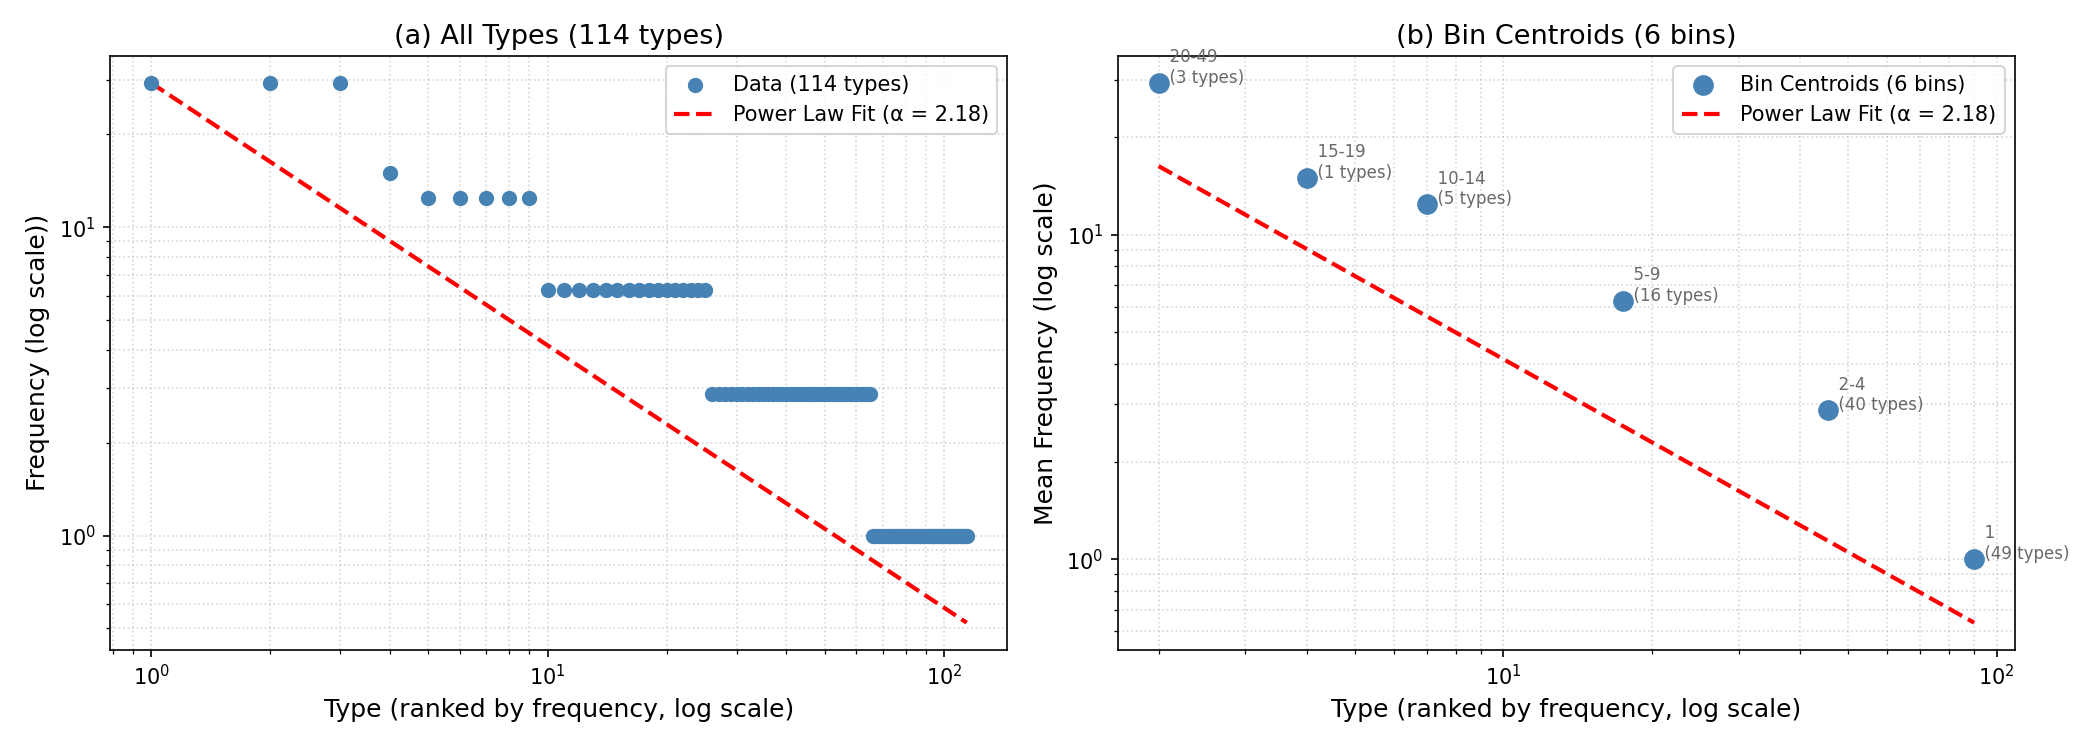
\includegraphics[width=\textwidth]{guilds.png}
    \caption{Log-log rank-frequency plot of offering stand styles (guild proxy). 
    (a)~All 114 types, showing stepped structure from binned data. 
    (b)~Bin centroids, showing the approximately linear log-log trend.}
    \label{fig:guilds}
\end{figure}

We note that if offering stand variation were purely artistic---reflecting individual 
craftspeople's aesthetic preferences---one would expect a roughly normal or Poisson 
distribution of styles. The power law distribution, with its characteristic heavy tail, 
instead implies a generative process involving growth and preferential attachment, consistent with 
the dynamics of market structures and organizational hierarchies \citep{axtell2001zipf}. 
The distribution type itself thus favors interpreting offering stand variants as markers 
of organizational identity rather than decorative choices.

\subsubsection{Constrained Reconstruction}

Jamison's text provides additional constraints beyond the binned table: the most common type 
(\#16) appears on 44 seals, only two other types (\#32 and \#44) exceed 20 seals (together 
totaling 44), and 49 types appear on exactly one seal \citep{jamison2017}. These constraints, 
combined with the bin boundaries and totals, allow us to generate plausible per-type frequency 
distributions via constrained random partitioning.

Across 5,000 such reconstructions (using discrete MLE fitting), the power law exponent was 
$\alpha = 2.49 \pm 0.14$ (median~2.54) with KS $D = 0.059 \pm 0.011$, dramatically 
improving the goodness-of-fit compared to the bin-mean approach ($D = 0.28$). A representative 
reconstruction (closest to median~$\alpha$) yields $\alpha = 2.36$, $D = 0.044$, and a 
bootstrap goodness-of-fit $p = 0.91$, well above the \citet{clauset2009power} threshold 
($p > 0.1$). While the likelihood ratio test favors the power law over the exponential
($R = 5.0$, $p = 0.295$), the difference is not statistically significant at this 
sample size. However, applying the \citet{clauset2009power} goodness-of-fit bootstrap to the 
exponential itself yields $p_{\text{GoF}} < 0.001$ (0/2500), formally ruling out the 
exponential as a plausible model for these data. No alternative heavy-tailed distribution 
fits significantly better.

Notably, the optimal lower bound is $x_{\min} = 1$, meaning the power law holds across 
the full range of guild sizes and all $n = 114$ types contribute to the tail fit---comfortably 
above the $n_{\text{tail}} \geq 100$ threshold recommended by \citet{clauset2009power} for 
reliable parameter estimation.

These results indicate that the poor goodness-of-fit obtained from bin means ($p < 0.01$) 
is entirely an artifact of the binning procedure, and that the underlying per-type guild 
size distribution is well described by a power law with $\alpha \approx 2.3$--$2.6$.

\subsection{Site Seal Distribution}

The distribution of seal counts across archaeological sites also follows a power law:

\begin{itemize}
    \item Power law exponent: $\alpha \approx 1.55$
    \item Lower bound: $x_{\min} = 2$ (5 single-seal sites excluded)
    \item KS distance: $D = 0.094$
    \item Goodness-of-fit $p = 0.76$ (bootstrap, 2500 iterations)
\end{itemize}

The fit is excellent ($D = 0.094$, $p_{\text{GoF}} = 0.76$) and significantly outperforms 
an exponential distribution ($R = 9.09$, $p = 0.019$). The high goodness-of-fit $p$-value 
means the power law cannot be rejected as a plausible generative model for the data 
\citep{clauset2009power}. The optimal lower bound is $x_{\min} = 2$; the power law holds across 
fourteen sites with 425 seals (5 single-seal sites excluded), which is well above the 
$n(\text{tail}) \geq 100$ threshold recommended by Clauset et al.\ \citep{clauset2009power}.

Table~\ref{tab:site_compare} summarizes the likelihood ratio tests against four alternative 
distributions.

\begin{table}[h]
\centering
\caption{Distribution comparison tests for site seal counts. 
Positive $R$ favors power law; negative $R$ favors the alternative.}
\label{tab:site_compare}
\begin{tabular}{@{}lrrl@{}}
\toprule
Alternative & $R$ & $p$ & Interpretation \\
\midrule
Lognormal & $-0.35$ & 0.520 & No significant difference \\
Exponential & 9.09 & 0.019 & Power law significantly better \\
Stretched exponential & $-0.39$ & 0.501 & No significant difference \\
Truncated power law & $-0.61$ & 0.271 & No significant difference \\
\bottomrule
\end{tabular}
\end{table}

\begin{figure}[h]
    \centering
    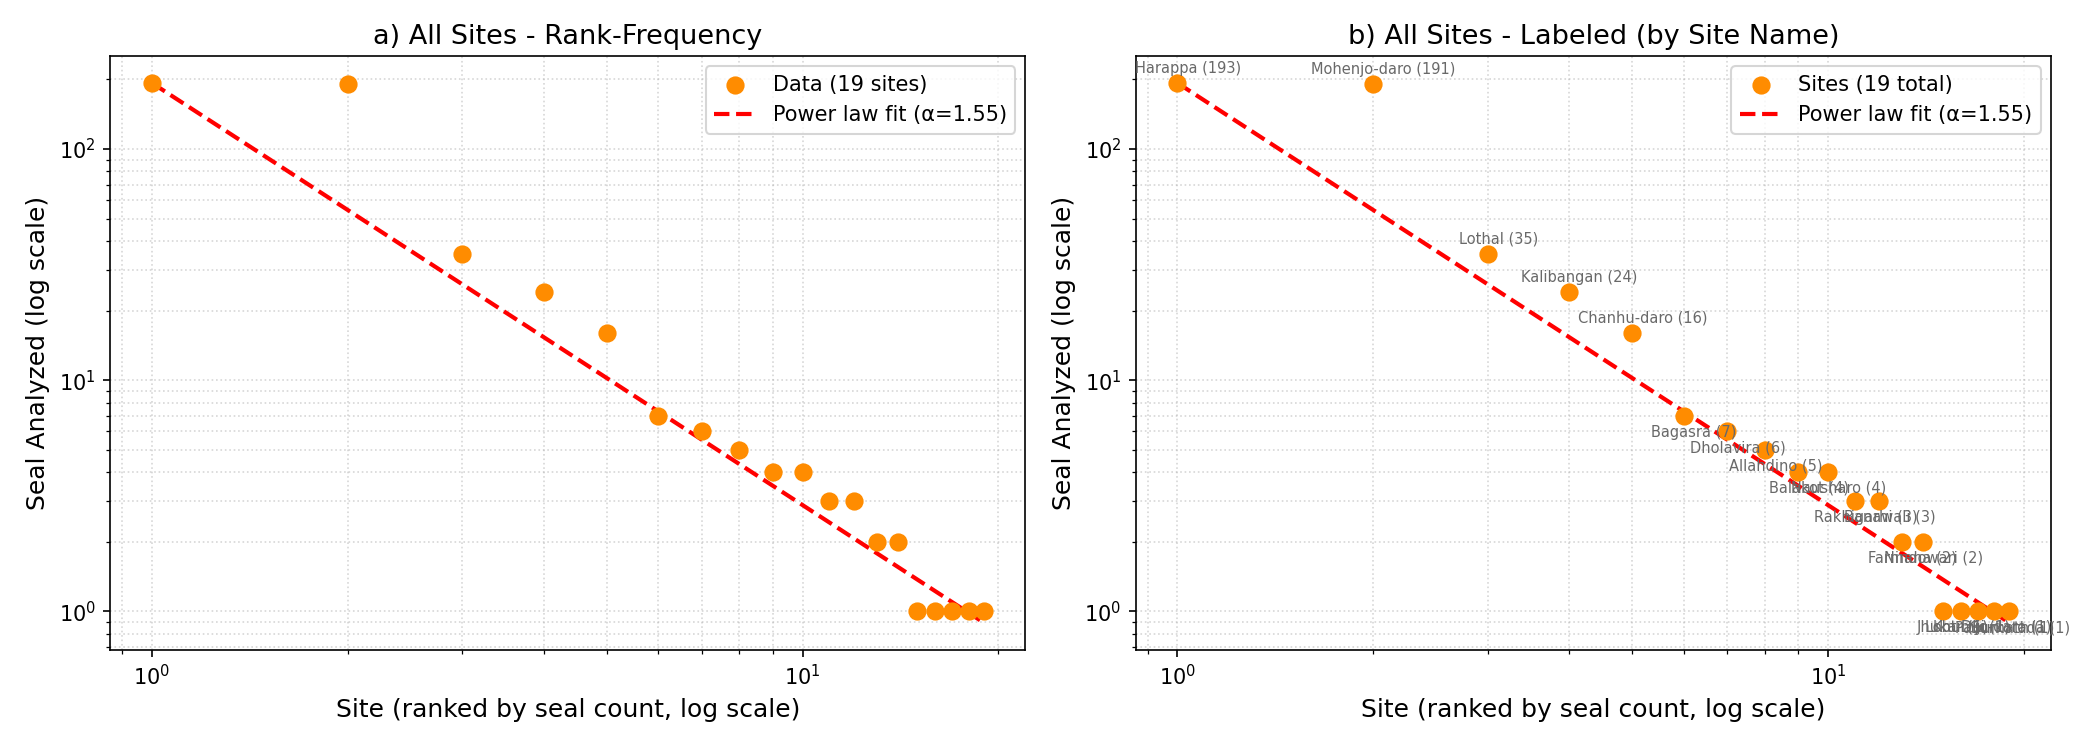
\includegraphics[width=\textwidth]{sites.png}
    \caption{Log-log rank-frequency plot of seal counts by archaeological site. 
    (a)~All 19 sites. (b)~Sites labeled with names and seal counts. Harappa and 
    Mohenjo-daro emerge as clear hub sites.}
    \label{fig:sites}
\end{figure}

The two most extensively excavated sites---Harappa (193 seals) and Mohenjo-daro 
(191 seals)---together account for 76.8\% of analyzed seals from only 10.5\% of sites. 
This concentration may partly reflect excavation history; sites such as Rakhigarhi, 
potentially the largest Harappan settlement by area, could alter the distribution as 
new seal data are published. The lower exponent ($\alpha \approx 1.55$) 
compared to the guild distribution reflects a heavier tail and even greater concentration at 
the site level: the top few cities are disproportionately dominant trade hubs.

\FloatBarrier
\subsection{Summary of Results}

\begin{table}[H]
\centering
\caption{Comparison of power law fits for guild and site distributions.}
\label{tab:comparison}
\begin{tabular}{@{}lccc@{}}
\toprule
Metric & Guilds (bin-mean) & Guilds (reconstructed) & Sites \\
\midrule
$\alpha$ & 2.18 & 2.49 $\pm$ 0.14 & 1.55 \\
$x_{\min}$ & 1.0 & 1.0 & 2.0 \\
KS $D$ & 0.28 & 0.059 $\pm$ 0.011 & 0.094 \\
GoF $p$ (bootstrap) & $<0.01$ & 0.91 & 0.76 \\
$R$ vs.\ exponential & 37.3 & 5.0 & 9.09 \\
$p$ vs.\ exponential & $<0.001$ & 0.295 & 0.019 \\
Exponential GoF $p$ & --- & $<0.001$ & --- \\
Data type & Binned & Constrained random & Exact \\
\bottomrule
\end{tabular}
\end{table}

\section{Discussion}

\subsection{A Scale-Free Harappan Trade Network}

Both distributions---guild sizes and site seal counts---exhibit the heavy-tailed, hub-dominated 
structure characteristic of scale-free networks. The evidence rests on two pillars:

\begin{enumerate}
    \item \textbf{Guild sizes follow a power law} ($\alpha \approx 2.3$--$2.6$ from 
    constrained reconstruction; bin-mean estimate $\alpha \approx 2.18$): A few dominant guilds 
    account for a disproportionate share of seals (the top 3 bins, representing 2.6\% of types, 
    account for 20.5\% of seals), while 49 guilds (43\% of types) appear only once.
    
    \item \textbf{Site seal counts follow a power law} ($\alpha \approx 1.55$): Two mega-hub 
    sites dominate the network. Preliminary evidence indicates that the top-ranked guild types 
    appear across most or all sites, consistent with hub guilds having high connectivity.
\end{enumerate}

\subsection{Reinterpreting Seal Iconography: Market Structure in the Offering Stand}

Jamison's typological work, building on foundational insights from Kenoyer \citep{kenoyer2000wealth}, 
interprets seal iconography variations through the lens of artisanal production and convincingly 
demonstrates that diversity reflects decentralization, not administrative standardization---a definitive 
finding we adopt entirely. Yet the distribution of offering stand variants reveals an additional layer: 
the frequency distribution follows a power law characteristic of scale-free networks associated with 
market structures and dynamics, suggesting that beneath artisanal variation lay a pre-structured market 
hierarchy.

The offering stand variants therefore represent merchant guild identities reflecting a market 
organization, not an artisanal development. The power law distribution indicates that the market 
was already differentiated into economic tiers: a few dominant guild types accounting for 
disproportionate volume across multiple sites, and a long tail of rare types. This market structure 
was encoded into the seal system itself through the offering stand variant, transforming what could 
otherwise appear as arbitrary carving variation into a standardized marker of guild identity and 
trading affiliation. The seal's multimodal information architecture thus operated at multiple levels: 
the unicorn motif identifies participation in the commercial network, the offering stand signals 
guild affiliation and market tier, and the script records transaction or administrative details.

\subsection{Corroborating Evidence: Jamison's Multi-Site Seal Groups}

Independent support for cross-site guild connectivity comes from Jamison's own grouping 
analysis. Using a composite criterion of at least seven shared attribute styles and five similar 
metric proportions, \citet{jamison2017} identified 55 seal groups comprising 180 seals (36\% 
of the sample). Table~\ref{tab:groups} reproduces the distribution of these groups by site.

\begin{table}[h]
\centering
\caption{Distribution of identified seal groups by site and count 
(reproduced from \citealt{jamison2017}, Table~9.1).}
\label{tab:groups}
\begin{tabular}{@{}lrr@{}}
\toprule
Site & Groups & Total Number of Seals in Groups \\
\midrule
Harappa        & 14 & 55 \\
Mohenjo-daro   & 16 & 51 \\
Kalibangan     & 2  & 4 \\
Lothal         & 1  & 4 \\
Bagasra        & 1  & 2 \\
Multiple Sites & 21 & 64 \\
\midrule
\textbf{Total} & \textbf{55} & \textbf{180} \\
\bottomrule
\end{tabular}
\end{table}

Notably, 21 of the 55 groups (38\%) span multiple archaeological sites, encompassing 64 seals. 
As \citet{jamison2017} notes, groups were found at 15 of the 19 sites in the sample. This cross-site grouping emerges 
despite the restrictive multi-attribute criterion; a grouping based solely on offering stand 
variant---as our model proposes---would be expected to yield broader geographic distributions, 
since it isolates the single attribute with maximal variation. The dominance of Harappa and 
Mohenjo-daro in the group counts further mirrors the hub structure identified in our 
site-level power law analysis.

\subsection{Implications for Civilization Dynamics}

Scale-free networks are robust to random failures but vulnerable to targeted disruption of hubs 
\citep{albert2000error}. Moreover, scale-free structure characteristically arises through growth and 
preferential attachment \citep{barabasi1999emergence}---a self-organizing process in which the network 
expands as new participants join and successful nodes attract disproportionately more connections over time. 
The Harappan Civilization's expansion over centuries across more than a million square kilometers, plausibly 
adding new guilds throughout, is consistent with such a self-organizing process. Notably, this mechanism requires 
no centralized seal production control, aligning with the IVC's apparent lack of centralized political authority 
\citep{possehl2002indus}.

This framework offers insight into both the longevity and decline of the IVC:

\begin{itemize}
    \item \textbf{Resilience} ($\sim$700 years of urban phase): Random loss of small guilds or 
    peripheral sites would have minimal impact on the overall trade network---a hallmark of 
    scale-free robustness.
    
    \item \textbf{Collapse}: Targeted disruption of hub guilds or hub sites---whether by 
    environmental stress (e.g., shifts in the Ghaggar-Hakra river system), disruption of 
    Mesopotamian trade routes, or other factors---could cascade through the network, causing 
    systemic failure disproportionate to the initial shock.
\end{itemize}

\subsection{Standardization Without Central Authority}

A long-standing puzzle in Harappan studies is the remarkable uniformity observed across the 
civilization---standardized brick ratios, weights, street grids, and seal formats---despite 
the apparent absence of a centralized state \citep{possehl2002indus}. The scale-free network 
model offers a parsimonious explanation. In networks dominated by a small number of hubs, 
the practices of those hubs naturally propagate to all connected nodes through repeated 
interaction. If the top guilds traded with partners across every major site, their norms 
regarding weights, measurement, and seal production would become \emph{de facto} standards 
without requiring top-down enforcement. Standardization, in this view, is an emergent property 
of hub-dominated trade rather than evidence of administrative control.

\subsection{The Disappearance of Unicorn Seals}

The scale-free framework also offers a structural account of the disappearance of unicorn 
seals during the Late Harappan phase. In a hub-dependent network, the collapse of a small 
number of dominant guilds would remove the nodes responsible for the majority of seal 
production and circulation. Within the analyzed unicorn seal system, 43\% of guild types appear 
only once; these marginal producers likely depended on the commercial infrastructure maintained 
by the hubs. Producers of non-unicorn seals, not systematically analyzed here, probably occupied 
similarly peripheral positions in the broader trade network. Once that infrastructure failed, the 
economic rationale for seal use---authentication of goods in a multi-party trade network---would 
have diminished. Sparse persistence of seals 
in outlying areas during the post-urban phase is consistent with the survival of peripheral 
nodes after hub removal, a well-characterized property of scale-free networks 
\citep{albert2000error}.

\subsection{Implications for Script Interpretation}

If the proposed information architecture is correct---unicorn as commercial network marker, offering 
stand as guild identifier, and script as the remaining variable element---then the script's function 
on seals may be more constrained than previously assumed. Rather than encoding open-ended 
linguistic content, the script in this context would serve to record transactional or 
administrative details associated with the sealed goods or secured context. This interpretation is agnostic to the broader question of whether the Indus 
script represents a full writing system or a more limited notational system; even a 
linguistic script could encode commodity names, quantities, or other administrative 
details. However, the seal's compact format 
and the brevity of most inscriptions (typically 4--5 signs) are consistent with a 
transactional function. Progress could come from correlating script sequences with offering stand 
variants. If signs co-vary with offering stand type, they likely encode guild-specific markers; 
if they are similar when guild-specific markers vary, they likely encode common information about 
commodities or administrative details. Additionally, site-specific guild markers could suggest 
commodities or administrative details specific to that site. We stress that this remains a hypothesis 
to be tested against the data, not a claim.

Independent support for this decomposition comes from \citet{mukhopadhyay2023}, who 
observes that seals from the same settlement frequently contain different iconographies but 
similar inscriptions---precisely the pattern predicted by our model, where a shared 
inscription encodes the same commodity or transaction while the differing iconographies 
identify different guilds trading in that commodity. More broadly, 
\citet{mukhopadhyay2023} independently concludes that Indus inscriptions encode trade and 
commodity control rather than proper nouns, and proposes that ``seal and tablet iconographies 
might have been the emblems of the guilds, rulers, and/or governing bodies''---a framing that 
aligns directly with the power law evidence for guild market structure presented here.

\subsection{Limitations}

The guild size analysis is based on binned summary data rather than per-type frequencies, 
which degrades the power law fit (KS $D = 0.28$ vs.\ $D = 0.094$ for the exact site data). 
A constrained reconstruction of per-type frequencies (Section~4.1.1) substantially mitigates 
this limitation, recovering $D = 0.059 \pm 0.011$ and an excellent goodness-of-fit 
($p = 0.91$), but exact per-type data would remove the need for reconstruction entirely. 
The sample of 500 seals represents approximately 39\% of the 1277 published unicorn seals and 
an unknown fraction of the total produced. More broadly, the Harappan Civilization has not 
been fully excavated: Possehl catalogs over 1,500 Harappan-period settlements, of which 
Jamison's sample covers only 19, and even major sites such as Rakhigarhi and Dholavira are 
only partially excavated. Additional data from ongoing and future excavations could 
strengthen or modify the power law fits presented here.

The guild interpretation is supported by convergent evidence: (1) the power law distribution 
argues against purely artistic variation, (2) concordance with modern firm size distributions 
\citep{axtell2001zipf}, and (3) Mukhopadhyay's independent findings on iconography function 
\citep{mukhopadhyay2023}. However, direct archaeological confirmation remains to be established.

\subsection{Future Work}

Direct archaeological confirmation of guild identities remains to be established through future 
investigation and discovery. Complementary quantitative work with exact per-type frequency data 
would enable:
\begin{itemize}
    \item A direct power law test for guild sizes, eliminating the need for constrained reconstruction
    
    \item Co-occurrence analysis and cross-site grouping based solely on offering stand type, enabling 
    reconstruction of the guild-level trade network. This could reveal the extent of top guild presence 
    across the network and where medium to small guilds operated.
    
    \item Archaeological confirmation linking specific offering stand variants to guild production and 
    trade identities.
\end{itemize}

\section*{Acknowledgments}

This work is deeply indebted to the meticulous typological scholarship of 
Gregg M.~Jamison, whose doctoral dissertation \citep{jamison2017} provided the 
comprehensive data on unicorn seal stylistic variation that made this analysis possible. 
Jamison's painstaking cataloguing of 500 seals across eleven attributes and nineteen 
archaeological sites represents years of careful archaeological work. While we reinterpret 
his data through a different analytical lens, we wish to emphasize that the empirical 
foundation is entirely his. Any errors in interpretation are our own.

Statistical analysis, code development, and manuscript preparation were assisted by 
GitHub Copilot (Claude, Anthropic).

\section{Conclusion}

Analysis of published Harappan seal data reveals that both the distribution of 
offering stand styles (a proxy for guild size) and the distribution of seals across archaeological 
sites are consistent with power law distributions, significantly outperforming exponential 
distributions---which is independently ruled out via its own goodness-of-fit bootstrap 
($p < 0.001$)---with no alternative heavy-tailed model fitting significantly better (lognormal, 
stretched exponential, truncated power law). A constrained reconstruction of per-type 
frequencies yields a guild size exponent of $\alpha \approx 2.3$--$2.6$ (bin-mean estimate 
$\alpha \approx 2.18$), within the canonical range for scale-free networks and 
consistent with modern firm size distributions. These findings support the hypothesis that 
the Harappan Civilization operated a self-organizing, scale-free commercial 
network---a structure that would explain both its remarkable longevity and its vulnerability to 
cascading failure. Exact per-type data and co-occurrence analysis would further strengthen 
these conclusions.

\bibliographystyle{plainnat}

\begin{thebibliography}{10}

\bibitem[Albert et al.(2000)]{albert2000error}
Albert, R., Jeong, H., \& Barab{\'a}si, A.-L. (2000).
\newblock Error and attack tolerance of complex networks.
\newblock {\em Nature}, 406(6794), 378--382.

\bibitem[Alstott et al.(2014)]{alstott2014powerlaw}
Alstott, J., Bullmore, E., \& Plenz, D. (2014).
\newblock powerlaw: A Python package for analysis of heavy-tailed distributions.
\newblock {\em PLoS ONE}, 9(1), e85777.

\bibitem[Ansumali Mukhopadhyay(2023)]{mukhopadhyay2023}
Ansumali Mukhopadhyay, B. (2023).
\newblock Semantic scope of Indus inscriptions comprising taxation, trade and craft 
licensing, commodity control and access control: archaeological and script-internal evidence.
\newblock {\em Humanities and Social Sciences Communications}, 10, 972.
\newblock \url{https://doi.org/10.1057/s41599-023-02320-7}

\bibitem[Axtell(2001)]{axtell2001zipf}
Axtell, R.~L. (2001).
\newblock Zipf distribution of U.S. firm sizes.
\newblock {\em Science}, 293(5536), 1818--1820.

\bibitem[Barab{\'a}si \& Albert(1999)]{barabasi1999emergence}
Barab{\'a}si, A.-L. \& Albert, R. (1999).
\newblock Emergence of scaling in random networks.
\newblock {\em Science}, 286(5439), 509--512.

\bibitem[Barab{\'a}si(2003)]{barabasi2003scale}
Barab{\'a}si, A.-L. (2003).
\newblock Scale-free networks.
\newblock {\em Scientific American}, 288(5), 60--69.

\bibitem[Clauset et al.(2009)]{clauset2009power}
Clauset, A., Shalizi, C.~R., \& Newman, M.~E.~J. (2009).
\newblock Power-law distributions in empirical data.
\newblock {\em SIAM Review}, 51(4), 661--703.

\bibitem[Jamison(2017)]{jamison2017}
Jamison, G.~M. (2017).
\newblock {\em The Organization of Indus Unicorn Seal Production: 
A Diachronic Comparative Study of Style, Skill, and Sociopolitical Organization}.
\newblock Ph.D.\ dissertation, University of Wisconsin--Madison.

\bibitem[Kenoyer(2000)]{kenoyer2000wealth}
Kenoyer, J. M. (2000).
\newblock Wealth and socio-economic hierarchies of the {I}ndus {V}alley civilization.
\newblock In J. Richards \& M. Van Buren (Eds.), {\em Order, legitimacy, and wealth in early states} (pp. 90--112).
\newblock Cambridge University Press.

\bibitem[Possehl(2002)]{possehl2002indus}
Possehl, G.~L. (2002).
\newblock {\em The Indus Civilization: A Contemporary Perspective}.
\newblock AltaMira Press.

\end{thebibliography}

\end{document}
